\documentclass[a4paper,12pt]{article}

\usepackage{../header}
\newcommand{\school}{ntu}
\newcommand{\subject}{math}
\renewcommand{\year}{106}
\newcommand{\titlename}{\MakeUppercase{\school} \subject \ \year}

\fancypagestyle{mainmatter}{\rhead{\titlename}}
\pagestyle{mainmatter}
\CenterWallPaper{.50}{img/logo_ntu_recolor.jpg}
\newcommand{\ver}{\textsc{Version} 1.0} % Version number.

\begin{document}

\title{\LARGE{\textbf{Solutions}} \\
	\Huge{\textbf{\titlename}} \\
	\normalsize{\ver}
}
\author{}
\date{}

\maketitle

% Start of solutions.

\begin{enumerate}
	\item \begin{answer}{$\dag$}\begin{equation}
            \begin{bmatrix}
                1 & 0 & 1 \\
                r & 1 & r \\
                3 & r & 2
            \end{bmatrix}    
        \end{equation}
    \end{answer}
    \item \begin{answer}{$\dag$}\begin{equation}
            2
        \end{equation}
    \end{answer} Since $\mat{A}$ has eigenvalues $0$ and $1$, it's \textbf{idempotent}, $\mat{A}^2 = \mat{A}$.
    \item Suppose \begin{equation}
        \mat{A} = \begin{bmatrix}
            x \\
            y
        \end{bmatrix}
    \end{equation} Then, we have projection \begin{equation}
        \mat{P} = \mat{A}(\mat{A}^\intercal\mat{A})^{-1}\mat{A}^\intercal
    \end{equation}
    \begin{answer}{$\dag$}\begin{equation}
            \frac{1}{x^2 + y^2}\begin{bmatrix}
                x^2 & xy \\
                xy & y^2
            \end{bmatrix}
        \end{equation}
    \end{answer}
    \item Suppose \begin{equation}
        \begin{cases}
            \beta & = \{(1, \ 0), \ (0, \ 1)\} \\
            \gamma & = \{\vec{u} = (1, \ 0), \ \vec{v} = (a, \ b)\}
        \end{cases}
    \end{equation} Then, we have \begin{equation}
        [x]_{\beta} = \begin{bmatrix}
            x_1 \\
            x_2
        \end{bmatrix}, \ [y]_{\beta} = \begin{bmatrix}
            y_1 \\
            y_2
        \end{bmatrix}, \ [x]_{\gamma} = \begin{bmatrix}
            s_1 \\
            s_2
        \end{bmatrix}, \ [y]_{\gamma} = \begin{bmatrix}
            t_1 \\
            t_2
        \end{bmatrix}
    \end{equation} Then ,we have transition matrix \begin{equation}
        \begin{aligned}
            & [\mat{I}]_{\gamma}^{\beta} = \begin{bmatrix}
                1 & a \\
                0 & b
            \end{bmatrix} \\
            \Rightarrow & \ [x]_{\beta} = \begin{bmatrix}
                s_1 + s_2a \\
                s_2b
            \end{bmatrix}, \ [y]_{\beta} = \begin{bmatrix}
                t_1 + t_2a \\
                t_2b
            \end{bmatrix}
        \end{aligned}
    \end{equation} Then, we have \begin{equation}
        \begin{aligned}
            f(\vec{x}, \vec{y}) & = (s_1 + s_2a)(t_1 + t_2a - t_2b) + s_2b \times (-t_1 - t_2a + 4 \times t_2b) \\
            & = s_1t_1 + s_2t_2 \\
            \Rightarrow & \ a = b = \pm \frac{1}{\sqrt{3}}
        \end{aligned}
    \end{equation}
    \begin{answer}{$\dag$}\begin{equation}
            \begin{bmatrix}
                1 & \frac{1}{\sqrt{3}} \\
                0 & \frac{1}{\sqrt{3}}
            \end{bmatrix} \lor \begin{bmatrix}
                1 & -\frac{1}{\sqrt{3}} \\
                0 & -\frac{1}{\sqrt{3}}
            \end{bmatrix}            
        \end{equation}
    \end{answer}
    \item We have pseudo-inverse \begin{equation}
        \mat{A}^{+} = (\mat{A}^\intercal\mat{A})^{-1}\mat{A}^\intercal
    \end{equation}
    \begin{answer}{$\dag$}\begin{equation}
            \begin{bmatrix}
                1 & 1 & 1 & 1 \\
                1 & 0 & -2 & 1 \\
                1 & -1 & 1 & 1
            \end{bmatrix}
        \end{equation}
    \end{answer}
    \item \begin{answer}{$\dag$}\begin{equation}
            2^{m^2} - 2^{m^2 - m} - 2^{m^2 - m} 
        \end{equation} Since both reflexive and irreflexive are $2^{m^2 - m}$.
    \end{answer}
    \item We have \begin{equation}
        \begin{aligned}
            & [(p \lor q) \land (\neg p \lor r)] \\
            \iff & \ (q \land \neg p) \lor (p \land r) \lor (q \land r) \\
            & \ \text{(Draw the Venn diagram)} \\
            \iff & \ (p \land r) \lor (\neg p \land q)
        \end{aligned}
    \end{equation} 
    \begin{answer}{$\dag$}\begin{equation}
            (p \land r) \lor (\neg p \land q)            
        \end{equation}
    \end{answer}
    \item We have \begin{equation}
        \begin{aligned}
            & \alpha^2 = \alpha + 1 \\
            \Rightarrow & \ \alpha = \frac{1 \pm \sqrt{5}}{2} \\
            \Rightarrow & \ a_n = c \times (\frac{1 + \sqrt{5}}{2})^n + d \times (\frac{1 - \sqrt{5}}{2})^n
        \end{aligned}
    \end{equation} And, we have \begin{equation}
        \begin{aligned}
            & \begin{cases}
                a_0 = c + d \\
                a_1 = c \times (\frac{1 + \sqrt{5}}{2}) + d \times (\frac{1 - \sqrt{5}}{2})
            \end{cases} \\
            \Rightarrow & \ c = \frac{2 \times a_1 - (1 - \sqrt{5})a_0}{2\sqrt{5}}, \ d = \frac{(1 + \sqrt{5})a_0 - 2 \times a_1}{2\sqrt{5}} \\
            \Rightarrow & \ a_n = \frac{2 \times a_1 - (1 - \sqrt{5})a_0}{2\sqrt{5}} \times (\frac{1 + \sqrt{5}}{2})^n + \frac{(1 + \sqrt{5})a_0 - 2 \times a_1}{2\sqrt{5}} \times (\frac{1 - \sqrt{5}}{2})^n
        \end{aligned}
    \end{equation}
    \begin{answer}{$\dag$}\begin{equation}
            A = 2 \times a_1 - (1 - \sqrt{5})a_0, \ B = 1 + \sqrt{5}, \ C = (1 + \sqrt{5})a_0 - 2 \times a_1, \ D = 1 - \sqrt{5}
        \end{equation}
    \end{answer}
    \item \begin{answer}{$\dag$} We have \begin{equation}
            \begin{aligned}
                & \gcd(n, n - 1) \\
                = & \ \gcd(n - 1, \ 1) \\
                = & \ 1
            \end{aligned}        
        \end{equation}
    \end{answer}
    \item \begin{answer}{$\dag$} bipartite
    \end{answer}
    \item We have \begin{equation}
        \begin{aligned}
            & 2^n = \binom{n}{0} + \binom{n}{1} + \cdots + \binom{n}{\frac{n - 1}{2}} + \binom{n}{\frac{n + 1}{2}} + \cdots + \binom{n}{n} \\
            \Rightarrow & \ \binom{n}{0} + \binom{n}{1} + \cdots + \binom{n}{\frac{n - 1}{2}} = \frac{2^n}{2} = 2^{n - 1}
        \end{aligned}
    \end{equation}
    \begin{answer}{$\dag$}\begin{equation}
            2^{n - 1}      
        \end{equation}
    \end{answer}
    \item \begin{answer}{$\dag$}\quad\begin{figure}[H]
            \centering
            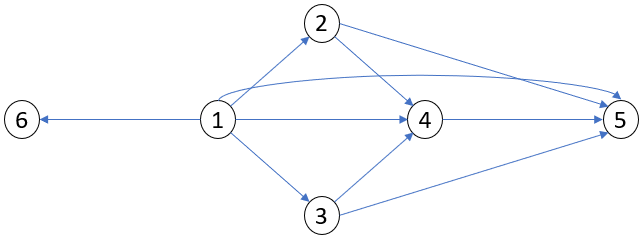
\includegraphics[scale=0.8]{img/ntu_106_math_12.png}
            \label{img:ntu_106_math_12}
        \end{figure}
    \end{answer}
\end{enumerate}

% End of solutions.

\end{document}
